\section{Exercise 4}
\subsection{Part a.}
Solve Eq.(1) using a tri-diagonal solver coded in python. A tri-diagonal
solver is a simplified Gaussian elimination solver that makes use of the
banded nature of the matrix to reduce the amount of storage and computation
required.

\begin{mdframed}[style=MyFrame]
    The following algorithm was used to solve the tri-diagonal system. 

    \begin{algorithm}[H]
        \DontPrintSemicolon
        \SetAlgoLined
        \KwResult{Calculating $d$}
        \SetKwInOut{Input}{Input}\SetKwInOut{Output}{Output}
        \Input{$a$, $b$, $c$, $d$}
        \Output{$d$}
        \BlankLine
            \For{ i in range(1,N)}{
                $m = a[i]/b[i]$\;
                $b[i] = b[i]-m*c[i]$\;
                $d[i] = d[i]-m*d[i]$\;
            }
            $d[-1] = d[-1]/b[-1]$\;
            \For{ i in range(N-2,-1, -1)}{
                $d[i] = (d[i]-c[i]*d[i+1])/b[i]$\;
            }
        \caption{Tri-diagonal solver subroutine}
    \end{algorithm}

    \emph{\textbf{See the appendix for the full python code}}
\end{mdframed}

\subsection{Part b.}
Plot the numerical solution (i.e, T(x) vs x) for $M = 4, 8, 16, 32, \text{
    and } 64$ alongside the exact analytical solution to Eq.(1). How does
the numerical result change with increasing mesh elements M ?
\begin{mdframed}[style=MyFrame]
    The temperature profile shown in Fig.~(\ref{fig:temperature-profile})
    clearly shows that the second order central difference method does
    accurately approximate the solution to the steady-state heat equation.  
    \begin{figure}[H]
        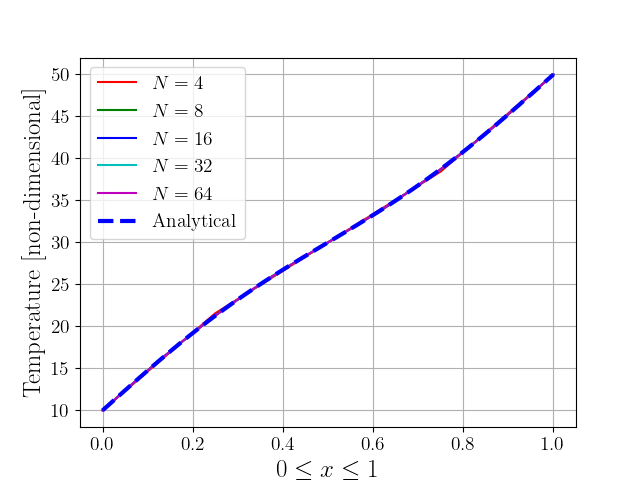
\includegraphics[height=0.35\textheight]{../media/temperature-profile.png}
        \caption{$T(x)$}
        \label{fig:temperature-profile}
    \end{figure}
    Furthermore, from the central difference method we know that the leading
    order truncation error is of order $O\left( \Delta x^{2} \right)$, namely  
    \begin{equation}       
        \dv[2]{f}{x} \approx \frac{f_{i+1} - 2 f_{i} + f_{i-1}}{\Delta x} 
                            + O\left(\Delta x^{2} \right)
    \end{equation}
    Therefore if we plot the error versus step size on a log-log plot we see
    that the error decreases with a slope of 2 since 
    \begin{equation}
        \log(e) = 2 \log\left(\Delta x \right)
    \end{equation}
    We can see this behavior in Fig~(\ref{fig:temp-error}), which would
    be a useful way to verify that we implemented our solver correctly and
    provide a tool to estimate the grid we would need for a certain error
    criteria. 
    \begin{figure}[H]
        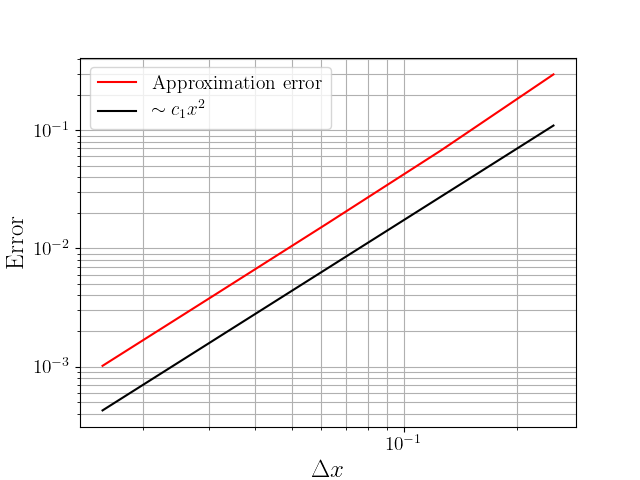
\includegraphics[height=0.35\textheight]{../media/error-profile.png}
        \caption{Error study}
        \label{fig:temp-error}
    \end{figure}
    \emph{\textbf{See the appendix for the full python code}}
\end{mdframed}

\subsection{Part c.}
Conduct a performance study on your tri-diagonal solver by solving Eq.(1)
with $M=10$, 100, 1000, 5000, 10000 elements and plotting mesh size versus
time. Briefly discuss your results.
\begin{mdframed}[style=MyFrame]
    In order to demonstrate the performance and the added benefit gained by
    using a tri-diagonal solver it makes the most sense to compare the time
    requirement to the perform $T=A^{-1}b$ using the following system,   
    \begin{equation}
        \begin{bmatrix}
            -2      & 1         &           &           &               &         \\  
            1       & -2        &   1       &           &               &         \\  
                    & 1         &   -2      &  1        &               &         \\  
                    &           &   1       &  -2       & \ddots        &         \\  
                    &           &           &  \ddots   & \ddots        & 1       \\  
                    &           &           &           & 1             & -2        

        \end{bmatrix}
        \begin{bmatrix}
            T_{1}       \\
            T_{2}       \\
            T_{3}       \\
            T_{4}       \\
            \vdots      \\
            T_{N-1}     \\
        \end{bmatrix}   
        =
        \Delta x^{2}
        \begin{bmatrix}
            Q_{1} + T_{0}/\Delta x^{2}      \\
            Q_{2}                           \\
            Q_{3}                           \\
            Q_{4}                           \\
            \vdots                          \\
            Q_{N-1} + T_{N}/\Delta x^{2}    \\
        \end{bmatrix}   
    \end{equation}
    Figures~(\ref{fig:time-comparison} \& \ref{fig:time-tri}) clearly show
    that there is a huge advantage in using a tri-diagonal solver compared
    to using the matrix inverse method. Furthermore, we can see in
    Fig.~(\ref{fig:time-ratio}) the for $M=10000$ the tri-diagonal vector
    method solves the systems $\sim \num{50e3}$ time faster then the matrix
    method. This should help build your understanding why we want to avaoid
    calculating the inverse of a matrix.
    \begin{figure}[H]
        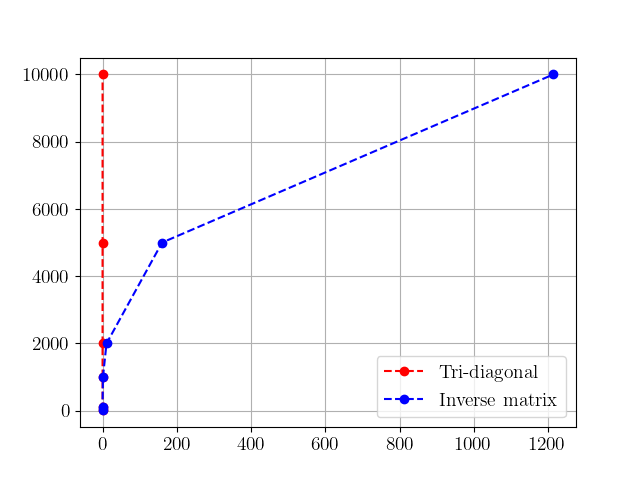
\includegraphics[height=0.35\textheight]{../media/time-comparison.png}
        \caption{Time study}
        \label{fig:time-comparison}
    \end{figure}
    \begin{figure}[H]
        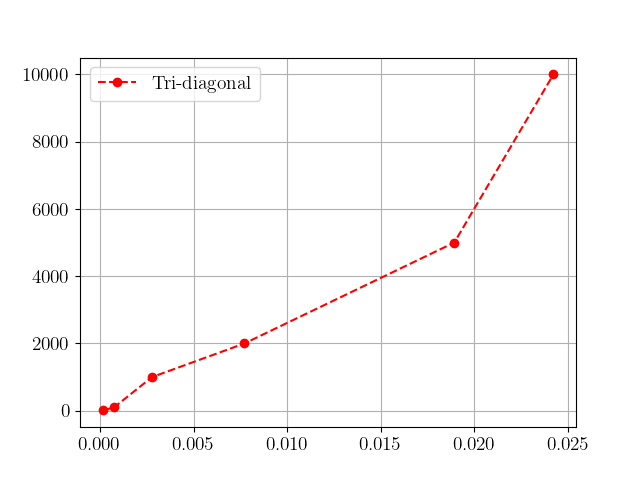
\includegraphics[height=0.35\textheight]{../media/tri-solve.png}
        \caption{Tri-diagonal time requirement}
        \label{fig:time-tri}
    \end{figure}

    \begin{figure}[H]
        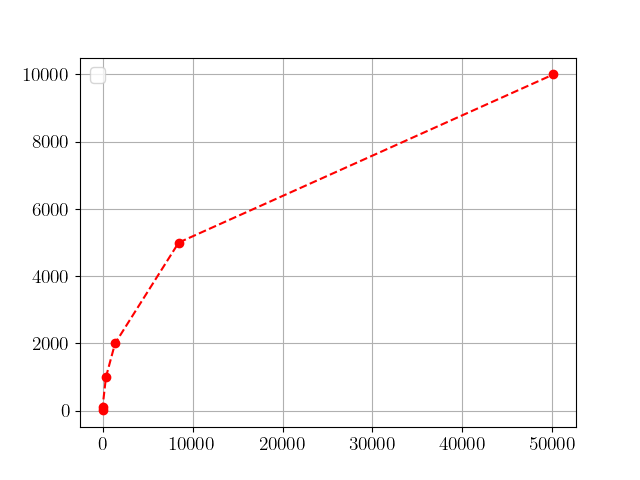
\includegraphics[height=0.35\textheight]{../media/time-ratio-solve.png}
        \caption{Ration between the inverse and tri-diagonal methods}
        \label{fig:time-ratio}
    \end{figure}
\end{mdframed}
